 \section{Results}
\label{sec:results}
In this Section we present some of the results obtained with our planner. The complete sequences computed are shown in the companion video, TODO.
Specifically, we demonstrate the planner for two really different robots, in a large vartiety of environments: the humanoid HRP-2 and the quadriped Hyq.
For each scenario we indicate the heuristics chosen. We also provide a performance analysis, that shows that the planner is compatible with interactive applications,
and present the success rates obtained in each scenario.
We also demonstrate the interest of our robustness criterion in the different computed poses.
Finally, a last example suggests possible applications to dextrous manipulation.

In our ISRR conference paper~\citep{tonneauisrr15}, additional results are demonstrated with various virtual avatars (Figure~\ref{fig:robots_old}).
In this extension we choose to focus on results obtained with actual robots. We invite the interested reader to watch the ISRR video\endnote{https://www.youtube.com/watch?v=LmLAHgGQJGA}, and 
to refer to the previous paper for a discussion on these results.

\begin{figure}[t]
\centering
  \begin{overpic}[width=1\linewidth]{figures/robots_old}
		%~ \put (5,58) {1)} 
		%~ \put (37,58) {2)} 
		%~ \put (68,58) {3.a)} 
		%~ \put (5,27) {3.b)} 
		%~ \put (37,27) {4.a)} 
		%~ \put (68,27) {4.b)} 
	\end{overpic}
\caption{Virtual avatars and associated volumes used in our conference paper: in red $W^0_{s}$; in green the range of motion of each limb.}
		   \label{fig:robots_old}
\end{figure}

\subsection{Description of the scenarios}
In all the scenarios considered, the formulation of the problem is always the same:
a start and goal root placements are provided as an input of the scenario.
The framework computes the initial balanced contact configuration, and outputs a sequence of statically balanced contact configurations connecting it to the goal.
A companion video available at TODO \url{http://youtu.be/LmLAHgGQJGA} (anonymous link) displays the complete contact sequence obtained in all these scenarios. The video only renders the contact configurations. Again, the interpolation between contact configurations is out of the scope of this paper~\citep{Carpentier2016}.

% \subsubsection*{Truck egress (Figure~\ref{res_truck_pres} and Figure~\ref{res_truck_bd}) -- Humanoid and insectoid robots.}
%\subsubsection*{Truck egress -- Humanoid and insectoid robots (Figure~\ref{res_truck_bd}).}
\noindent\textbf{Truck egress (humanoid and insectoid):}
The robot must leave a truck the doors of which are blocked: it has to crawl through the front window.
Figure~\ref{res_truck_bd} presents the sequence of contacts obtained for both robots: RB-PRM can find solutions in highly cluttered environments with narrow passages.

\begin{figure}[h!]
  \centering
  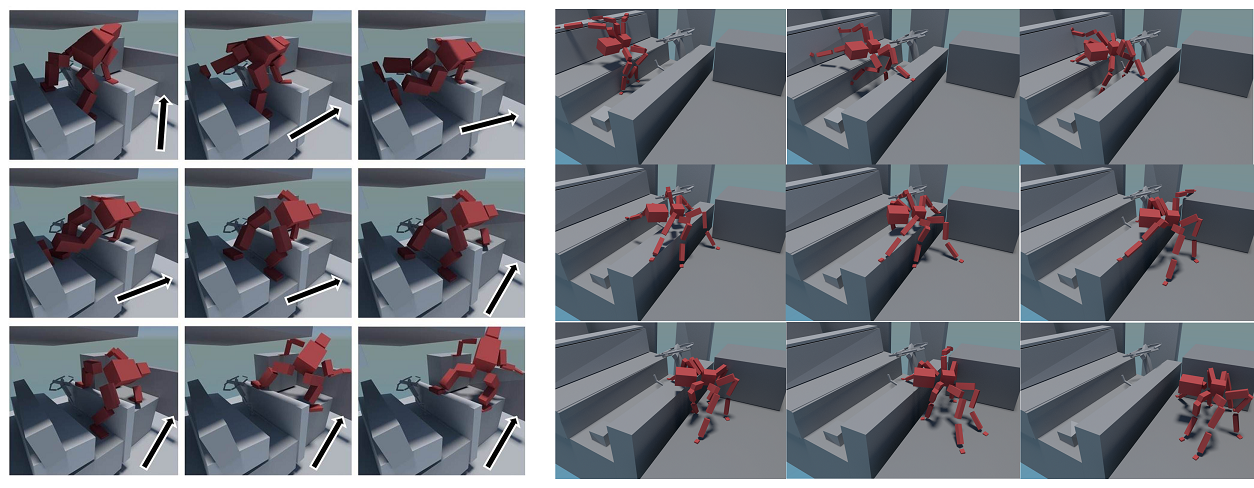
\includegraphics[width=1\linewidth]{figures/climballlow}
  \caption{
           The computed contact sequences for the truck egress scenario. Only selected postures are shown for the insect.}
		   \label{res_truck_bd}
\end{figure}

% \subsubsection*{Climbing (Figure~\ref{res_climb}) -- Humanoid and insectoid robots.}
%\subsubsection*{Climbing -- Humanoid and insectoid robots.}
\noindent\textbf{Climbing (humanoid and insectoid):}
The robot has to climb on a wall with several grasps disposed along it. In this scenario, we give stronger conditions for the sampled root placements: we require that more than one range of motion $W^k$ collide with obstacles of the environment. Fig.~\ref{res_climb} presents the contact sequence obtained for the 
humanoid robot.

\begin{figure}[h!]
  \centering
  %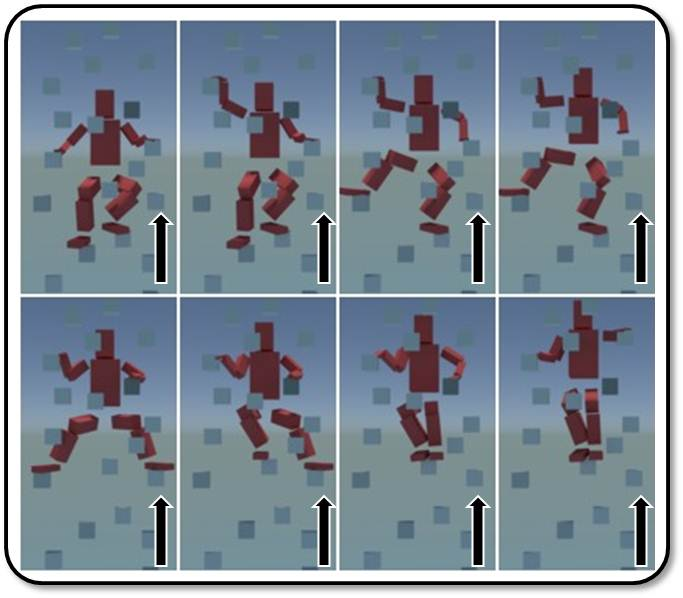
\includegraphics[width=0.6\linewidth]{figures/climb}
  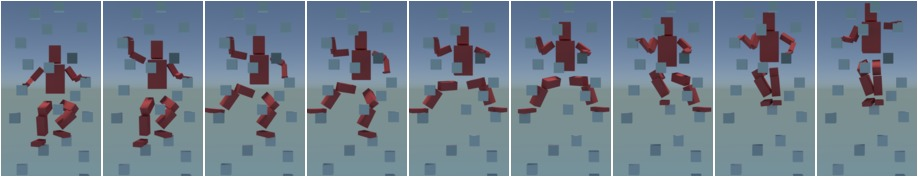
\includegraphics[width=1\linewidth]{figures/climb_line}
  \caption{The computed sequence for the climbing scenario.}
		   \label{res_climb}
\end{figure}


%~ \subsection{Implementation details}
%~ The test application was developed using the C++ language.
%~ The volumes describing the Range Of Motions of the robots $A_{ROM}$ are computed using the Matlab mpt toolbox~\footnote{http://people.ee.ethz.ch/\~mpt/3/}.
%~ They are exported to the obj format using a custom Matlab script.
%~ 
%~ The robot is described using the urdf file format~\footnote{http://wiki.ros.org/urdf}, used as a standard by the popular ROS platform.
%~ The scenarios where described using a custom text file format.
%~ Environments are described in the obj format. Rendering is achieved using Blender~\footnote{http://www.blender.org}.
%~ The runs were performed on a laptop with an Intel Core i7-2760QM 2.40GHz processor and 4 GB of memory. The application is not multi-threaded.

\noindent\textbf{Manipulation of a pen (3-finger hand):}
This scenario is proposed to illustrate the genericity of our approach: we consider a manipulation task for a robotic hand and use
our contact planner to compute a guide trajectory for the fingers, considered as effectors (Figure \ref{fig:penrot}).
Although we do not address the hard issue of accounting for rolling motions, the planner is able to compute the shown sequences, this in less than 5 seconds.

\begin{figure}[t]
\centering
  \begin{overpic}[width=1\linewidth]{figures/penrot}
	\end{overpic}
\caption{Contact sequence found for a pen manipulation in a zero gravity environment.}
		   \label{fig:penrot}
\end{figure}
 
%\subsubsection*{Other scenarios}
\noindent\textbf{Other scenarios (humanoids): }
%Two additional scenarios were considered for the humanoid robot. A crouching scenario, and a standing up scenario (already presented in Figure~\ref{fig:framework} -- right) -- Humanoid robot). 
The standing-up scenario (already presented in Fig.~\ref{fig:framework}) is a setup taken from \cite{DBLP:conf/iser/EscandeKMG08}: it corresponds to a long narrow passage in the configuration space.
In the crouching scenario, demonstrated in the companion video, the character automatically goes from a standing to a crouching position to crawl under an obstacle.



\subsection{Parametrization of the reachability condition} \label{sec:stat1}


To find the appropriate $C_{reach}^s$ in which to sample the guide trajectory,
we computed the rejection rate for various values of $s$ for each robot in the most cluttered truck scenario.
For a given value of $s$, $10^6$ root positions and orientations are computed
in $C_{reach}^s$. In each case we try to generate a collision free contact configuration, with a database
comprising $N=10^5$ sample configurations for each limb. The rejection rate
is the ratio between the number of failures  and the number of trials. From Figure~\ref{fig:rejection} $s$ is empirically chosen
as the smallest value for which the rejection rate is minimal.
For the humanoid, we thus chose $s=2.2$, and for the insect, $s=2.8$.

\begin{figure}[t]
\centering
  \begin{overpic}[width=0.6\linewidth]{figures/rejectionnotext}
		 \put (1.1,24){\rotatebox{90}{\tiny{Rejection rate}}}
		 \put (4.8,52) {\tiny{20} }
		 \put (4.8,48) {\tiny{18} }
		 \put (4.8,43) {\tiny{16} }
		 \put (4.8,38) {\tiny{14} }
		 \put (4.8,34) {\tiny{12} }
		 \put (4.8,29) {\tiny{10} }
		 \put (4.8,24.5) {\tiny{8} }
		 \put (4.8,20) {\tiny{6} }
		 \put (4.8,15) {\tiny{4} }
		 \put (4.8,10) {\tiny{2} }
		 \put (11.5,5) {\tiny{1} }
		 \put (24.5,5) {\tiny{1.5} }
		 \put (39,5) {\tiny{2} }
		 \put (52,5) {\tiny{2.5} }
		 \put (45,3) {\tiny{s} }
		 \put (66,5) {\tiny{3} }
		 \put (79,5) {\tiny{3.5} }
		%~ \put (37,58) {2)} 
		%~ \put (68,58) {3.a)} 
		%~ \put (5,27) {3.b)} 
		%~ \put (37,27) {4.a)} 
		%~ \put (68,27) {4.b)} 
	\end{overpic}
\caption{Truck scenario rejection rates(\%) for the humanoid(orange) and insectoid(blue), given $s$.}
		   \label{fig:rejection}
\end{figure}




\subsection{Performance}\label{sec:stat2}
The number of samples used for generating the contacts of each limb is 10000.
Table~\ref{tab:requestime} presents the average time (seconds) spent in the phases of the planner, for 
each phase and each scenario, and the number of contact phases of the sequence.

\begin{table}[b]
\centering
\begin{tabular}{ l | >{\centering\arraybackslash}m{65pt} | >{\centering\arraybackslash}m{65pt} | >{\centering\arraybackslash}m{65pt} | c}
  &  Generate RB-PRM (offline) & Generating the contact sequence & Number of contact states\\
 \hline
   Truck egress (humanoid) & $ 73 $ & 15 & 10 \\
   Truck egress (insectoid) & $70$ & 23 & 48\\
   Climbing (humanoid)& $25$ &  5 & 15\\
   Climbing (insectoid)  & $ 21 $ & 27 & 51\\
   Crouching (humanoid)& $5$ & 6 & 22 \\
 \end{tabular}
\caption{\textbf{Average time} (in seconds) spent in RB-PRM generation, and the online generation of the contact sequence.}
\label{tab:requestime}
\quad
 \end{table}

 We observe that many contacts are required for the insect, which can be explained by its restricted range of motion.
 The time spent generating the navigation graph is about one minute. The time spent in generating the graph of the climbing scenario,
 despite the relatively open environment, is explained by the additional restrictions imposed on the reachability condition.
 The difficulty to find a balanced configuration essentially influences the time spent generating the contacts.
 
The number of contacts in the sequence gives a rough estimation of its duration in seconds. Except for the robots crawling out of the truck, all the contact generation are real-time. Additionaly to the quality of the generated trajectories shown in the video, these computation times are a major practical achievement. 


%~ \subsection{Early results: manipulating scenario in zero gravity}
%~ In this scenario, we suggest an extension of our framework to manipulation.
%~ We consider the task of rotating a pen using a robotic hand.
%~ A start and goal configurations for the pen are expressed in the world coordinate system.
%~ The problem is automatically reformulated into an equivalent motion planning one for the robotic hand, by expressing its start
%~ and goal configurations in the coordinate system of the pen. In other words, for the planning the pen is considered as a static object, and a feasible motion for the hand
%~ is computed along the pen. Figure {penrot} presents the results obtained with this approach.
%~ Additional work is required to generate feasible manipulation motions.
